\documentclass[a4paper,10pt]{article}
\usepackage{%
	amsmath,%
	amsfonts,%
	amssymb,%
	amsthm,%
	hyperref,%
	url,%
	latexsym,%
	epsfig,%
	graphicx,%
	psfrag,%
	subfigure,%	
	color,%
	tikz,%
	pgf,%
	pgfplots,%
	pgfplotstable,%
	pgfpages%
}

\usepgflibrary{shapes}
\usetikzlibrary{%
  arrows,%
	backgrounds,%
	chains,%
	decorations.pathmorphing,% /pgf/decoration/random steps | erste Graphik
	decorations.text,%
	matrix,%
  positioning,% wg. " of "
  fit,%
	patterns,%
  petri,%
	plotmarks,%
  scopes,%
	shadows,%
  shapes.misc,% wg. rounded rectangle
  shapes.arrows,%
	shapes.callouts,%
  shapes%
}

\newcommand{\beq}{\begin{equation}}
\newcommand{\eeq}{\end{equation}}
\newcommand{\beqn}{\[}
\newcommand{\eeqn}{\]}
\newcommand{\bea}{\begin{eqnarray}}
\newcommand{\eea}{\end{eqnarray}}
\newcommand{\bean}{\begin{eqnarray*}}
\newcommand{\eean}{\end{eqnarray*}}
\newcommand{\re}{\mbox{$\mathfrak{Re}$}}
\newcommand{\bit}{\begin{itemize}}
\newcommand{\eit}{\end{itemize}}
\newcommand{\ben}{\begin{enumerate}}
\newcommand{\een}{\end{enumerate}}

\theoremstyle{plain}
\newtheorem{thm}{Theorem}[section]
\newtheorem{lem}[thm]{Lemma}
\newtheorem{prop}[thm]{Proposition}
\newtheorem{cor}[thm]{Corollary}

\theoremstyle{definition}
\newtheorem{defn}[thm]{Definition}
\newtheorem{conj}[thm]{Conjecture}
\newtheorem{exmp}[thm]{Example}

\theoremstyle{remark}
\newtheorem{rem}[thm]{Remark}
\newtheorem{note}[thm]{Note}

\date{}
\title{Lecture 3:  Compound Poisson Processes}
\author{Parimal Parag}

\begin{document}
\maketitle

\subsection{Conditional Distribution of the Arrival Instants}
\noindent For the Poisson process $\{N_{t}, t\geq 0\}$ with rate $0<\lambda< \infty$, we would like to find the density.
\begin{eqnarray*}
% \nonumber to remove numbering (before each equation)
  P(S_{1}\mid N_{t}=1), t>0 \\
  P_{S_1}(S \mid N_{t}=1) \\
  P(s\leq S_{1} \leq s+h \mid N_{t}=1)\\
   &\approx& h P_{S_1}(S \mid N_{t}=1 \\
  P(s\leq S_{1}< s+h \mid N_{t}=1)\\
   &=& \frac{P(s\leq S_{1}< s+h,N_{t}=1)}{P(N_{t}=1)}\\
   &=& \frac{P[s\leq S_{1}<s+h,X_{2}>t-(s+h))}{\lambda t e^{-\lambda t}} \\
   &=& \frac{h \lambda e^{-\lambda h} e^{-\lambda (t-(s+h))}}{h{\lambda t} e^{-\lambda t}}.
   \end{eqnarray*}
   Take  $\lim _{h\rightarrow 0}\frac{1}{t}{e^{-\lambda h}} =\frac{1}{t}.$ Thus, the conditional density is the density of a uniform random variable distributed over the interval $[0,t].$ This property of Poisson process can be generalized. For $0<s_{1}<s_{2},.., s_{n}<t$ and $n=1,2 \hdots$ \\

\begin{eqnarray*}
% \nonumber to remove numbering (before each equation)
    &P[s_{1}\leq S_{1}<s_{1}+h, s_{2}\leq S_{2}<s_{2}+h, ...s_{n}\leq S_{n}\leq s_{n}+h \mid N_{t}=n]  \\
   &=   \frac{P[s_{1}\leq S_{1}<s_{1}+h, s_{2}\leq S_{2}<s_{2}+h,...,s_{n}\leq S_{n}\leq s_{n}+h,N_{t}=n]}{P[N_{t}=n]} \\
   &=  \frac{P[s_{1} \leq S_{1}<s_{1}+h_{1},s_{2}-s_{1}\leq X_{2}<s_{2}- (s_{1}+h),..., X_{n+1}> t-s_{n}]}{P[N_{t}=n]} \\
   &\stackrel{(a)}{=}  \frac{P[s_{1 \leq S_{1}<s_{1}+h}]P[s_{2}-s_{1}\leq X_{2}<s_{2}-s_{1}+h] P[X_{n+1}>t -s_{n}]}{P[N_{t}=n]}\\
   &=  \frac{\lambda h e^{-s_{1}\lambda}h \lambda e^{-(s_{2}-s_{1})\lambda},..., e^{-(t-s_{n})\lambda}}{(\lambda t)^{n}\frac{e^{-\lambda t}}{n!}} 
   \end{eqnarray*}
   \begin{eqnarray*}
    \lim _{h\rightarrow 0} \frac{ \lambda h e^{-s_{1}\lambda}h \lambda e^{-(s_{2}-s_{1})\lambda},... e^{-(t-s_{n})\lambda}}{h^{n}(\lambda t)^{n}\frac{e^{-\lambda t}}{n!}}=\frac{n!}{t^{n}}.
\end{eqnarray*}
where (a) follows as $X_i$s are independent. Thus, if $U_{1},... U_{n}$ are $iid$ Uniform random variables in $[0,t]$, conditioned on $\{N_t=n\}$, the $n$ arrival instants have the same distribution as the order statistics  of $U_1 \hdots U_n$.\\
We give some more properties of the Poisson process. \\
Suppose, ${N_{1 }(t), t \geq  0}$ Poisson process unit rate $\lambda _{1}$, ${N_{2} (t), t \geq  0}$ Poisson process unit rate $\lambda _{2}$. Further, assume that the two Poisson processes are independent of each other. Let $N(t)= N_{1}(t) +N_{2}(t)$. \\

\textbf{Claim}: ${N(t), t \geq  0}$ is a Poisson process with rate $\lambda_{1}+\lambda_{2}$.\\ 
\textbf{Proof}: Need to show that
\begin{eqnarray*}
% \nonumber to remove numbering (before each equation)
 \frac{P[Nt=n]  [(\lambda_{1}+\lambda_{2}t]^{n}e^{-\lambda_{1}+\lambda_{2}t}}{n!}\\
\end{eqnarray*}
and $\{N_t\}$ has stationary, independent increments.\\
For $N_{1}(t)$,  arrivals in $(t_{1}, t_{2})\perp (t_3,t_{4})$. Similarly, for $N_{2}(t)$ arrivals in $(t_{1}, t_{2})\perp (t3,t_{4})$. Therefore, $N(t)$ has independent increment property. Similarly, we can argue out stationary increment property of $\{N_t\}$.\\
\begin{eqnarray*}
% \nonumber to remove numbering (before each equation)
  P[N(t)=n] &=& P[N_{1}(t)+ N_{2}(t)= n] \\
   &=& \sum_{n1} P [N_{1}(t)=n_{1},N_{2}(t)= n-n_{1} ] \\
  &=& \sum_{n_{1}}\frac{e^{-\lambda _{1}t}(\lambda_{1}t)^{n_{1}}}{n_{1}!}e^{-\lambda_{2}t}\frac{(\lambda_{2}t)^{(n-n_{1})}}{(n-n_{1})!} \\
   &=&\sum_{n_{1} (\lambda _{2}t)} \frac{e^{-(\lambda_{1}+\lambda_{2})t} (\lambda_{1}t)^{n1}(\lambda_{2}t)^{-n_{1}}}{n_{1}! (n-n_{1})!} \\
   &=& \frac{e^{-(\lambda_{1}+\lambda_{2})t}}{n!}\sum^{n}_{n_{1=0}}\left(\frac{\lambda_{1}}{\lambda_{2}}\right)^{n_{1}}\left(\frac{\lambda_{2}}{n_{1}!}\right)^{n}\frac{n!}{(n-n_{1})!} \\
   &=&  \frac{e^{-(\lambda_{1}+\lambda_{2})t}}{n!}(\lambda_{1}+\lambda_{2})^{n}t^{n}
\end{eqnarray*}
\begin{figure}
\centering
  % Requires \usepackage{graphicx}
  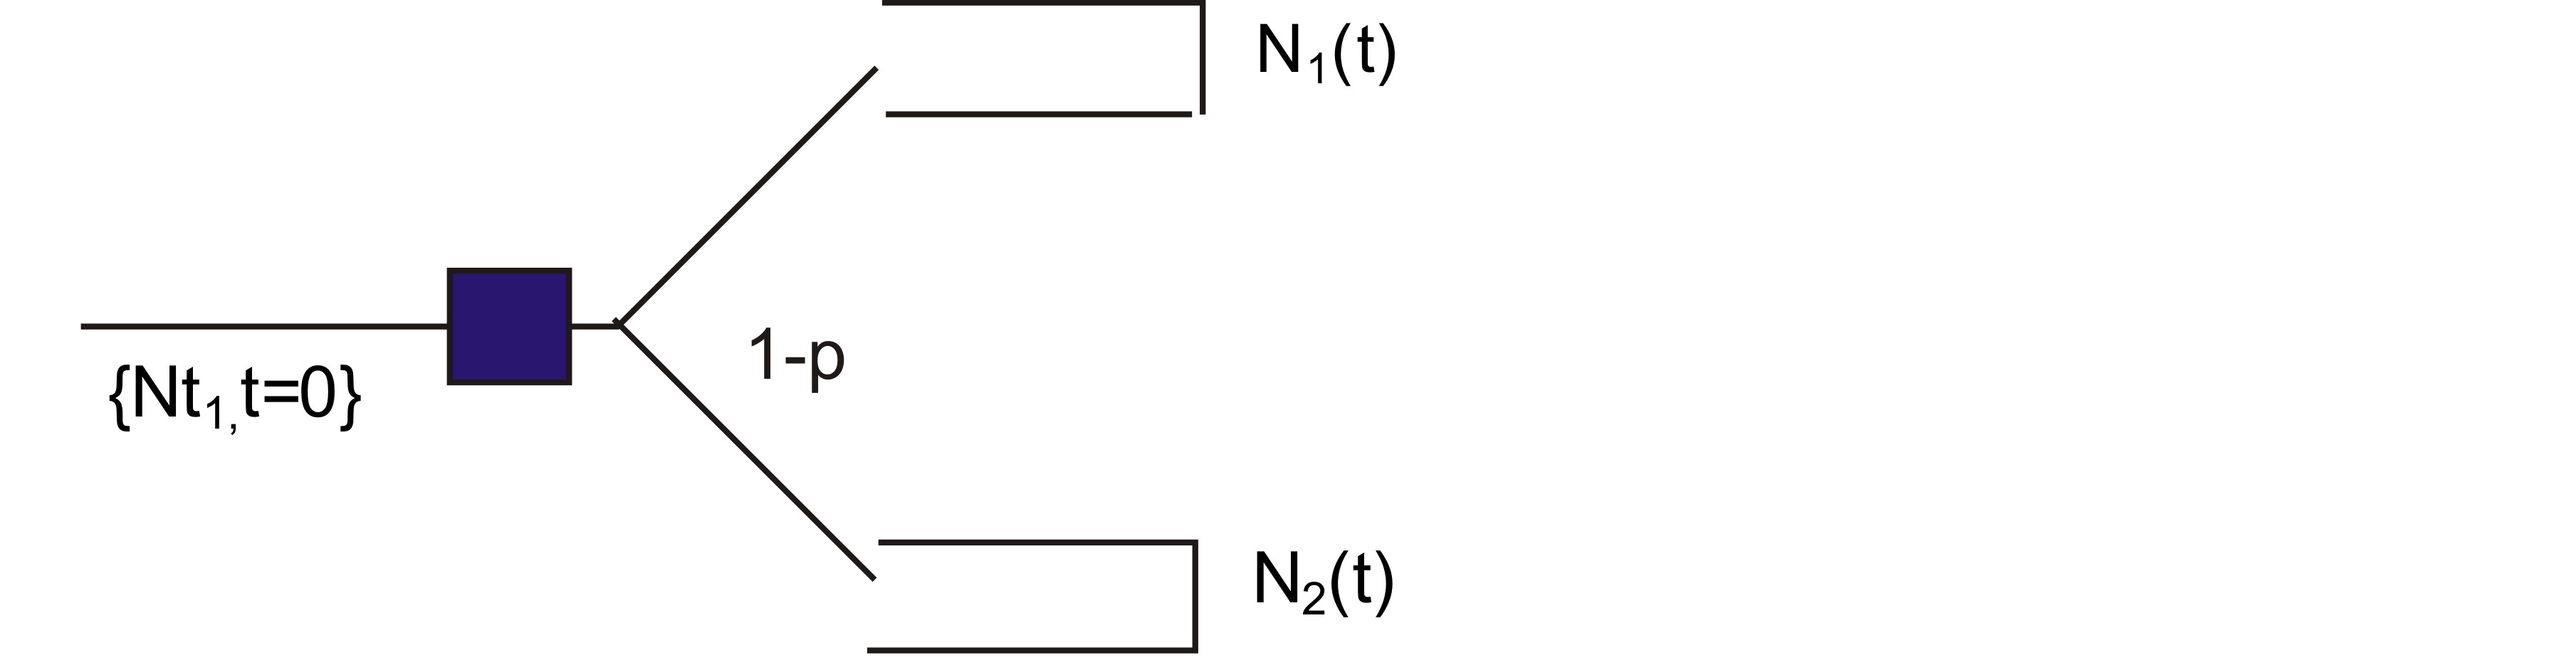
\includegraphics[width=5.0in]{Figures/comment.PNG}\\
 % \caption{}\label{}
\end{figure}

\textbf{Comment}: If independence condition is removed, the statement is not true.\\

\textbf{Claim}:${N_{1}(t), t\geq 0}, {N_{2}(t), t \geq 0}$ are Poisson processes with rates $\lambda p$ and $\lambda (1-p)$ and these process are independent of each other.  

\textbf{Proof:} To show that ${N_{1}(t), t \geq 0}$ is a Poisson process with rate $\lambda p$, we show that it is stationary independent increment process with the distribution
\begin{eqnarray*}
% \nonumber to remove numbering (before each equation)
 P[N_{1}(t)= n]  = \frac{(p \lambda t)^{n}}{n!}e^{-\lambda p t}.
\end{eqnarray*}
\begin{figure}
\center
  % Requires \usepackage{graphicx}
  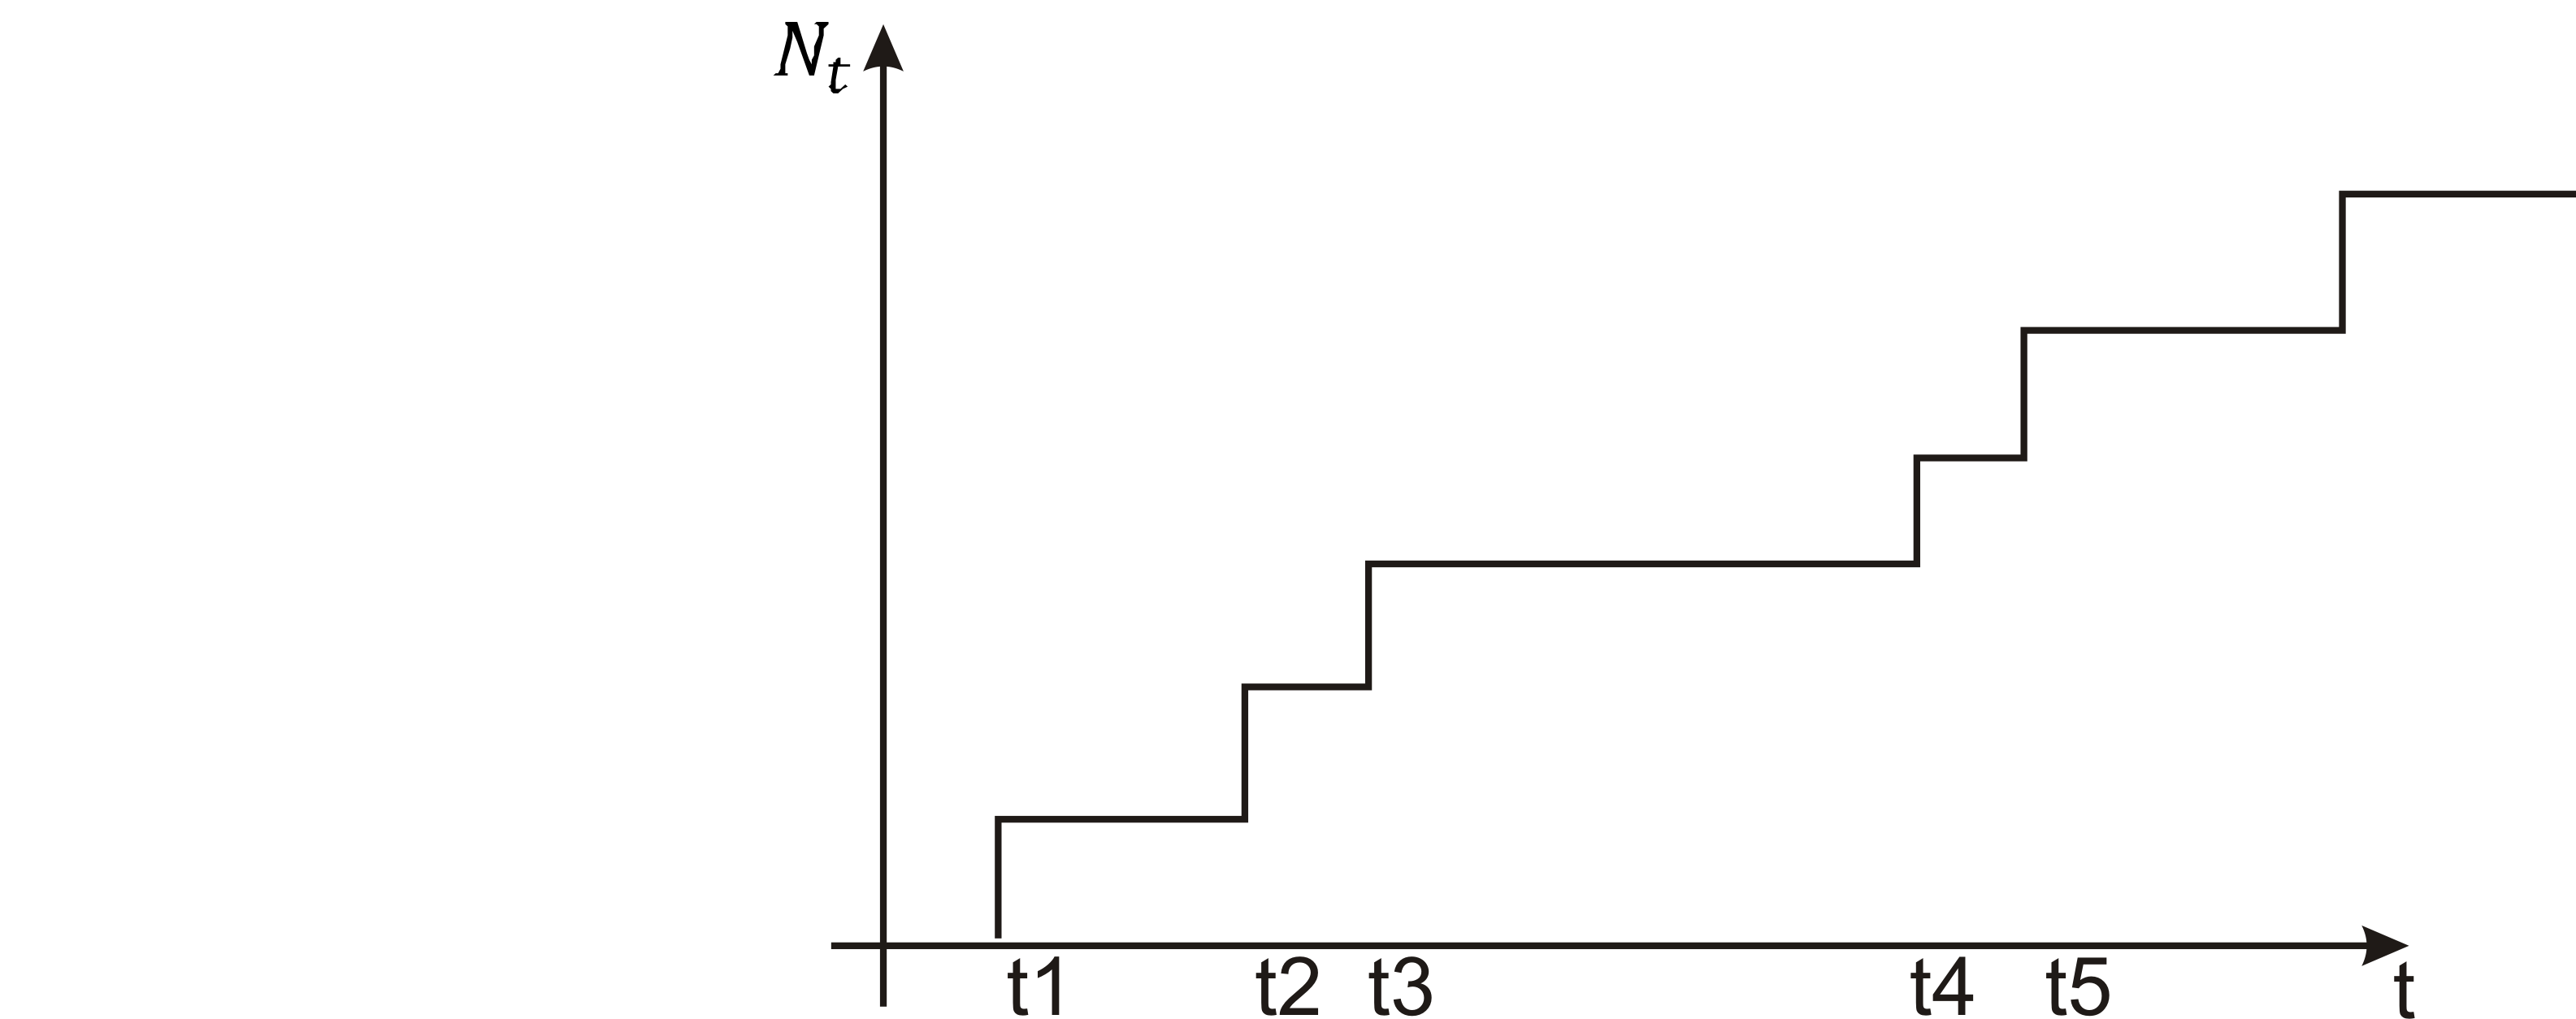
\includegraphics[width=4.5in]{Figures/distr.PNG}\\
 % \caption{}\label{}
\end{figure}
The stationary, independent increment property of the probabilistically filtered processes $\{N_1(t)\}$ and $\{N_2(t)\}$ can be understood and argued out from the example given in the figure. \\
  \begin{eqnarray*}
  % \nonumber to remove numbering (before each equation)
    P[N_{1}(t) =n]&=& \sum^{\infty}_{m=0}P[N(t)=m, N_{1}(t) = n]  \\
   &=& \sum^{\infty}_{m=n}P[N(t)=m] p^{n}(i-p)^{m-n}mC_n\\
   &=&  \sum^{\infty}_{m=n}\frac{e^{-\lambda t(\lambda t)^{m}}}{m!}p^{n}(1-p)^{m-n}(mC_n)\\
     &=& e^{-\lambda t}p^{n}\sum_{m=n}\frac{(\lambda t)^{m-n}}{m!}\frac{(1-p)^{m-n}m!}{n!(m-n)!} \\
     &=& \frac{e^{-\lambda t p}(p \lambda t)^{n}}{n!} \sum^{\infty}_{m=n}e^{-\lambda (1-p)t}\frac{(\lambda (1-p)t)^{m-n}}{(m-n)!} \\
     &=&  \frac{e^{-\lambda t p}(p \lambda t)^{n}}{n!} \sum^{\infty}_{k=0}e^{-\lambda (1-p)t}\frac{(\lambda (1-p)t)^{k}}{k!}  \\
     &=& \frac{e^{-\lambda p t}(p \lambda t)^{n}}{n!}.
  \end{eqnarray*}
To show that 
\begin{eqnarray*}
% \nonumber to remove numbering (before each equation)
   \{N_{1}(t), t \geq 0\}&\perp&\{N_{2}(t), t \geq 0\}  \\
   P[N_{1}(t)&=&n_{1}, N_{2}(t) = n_{2}]\\
    P[N(t) = n_{1}+ n_{2}]&=& \frac{e^{-\lambda t} (\lambda t)^{n_{1}+n_{2}}}{(n_{1}+n_{2})!} \\
   &=&  \frac{e^{-\lambda p t}e^{-\lambda (1-p)t}}{(n_{1}+n_{2})!} -(\lambda t)^{n_{1}+n_{2}}\\
   &=&  \frac{e^{-\lambda p t}e^{-\lambda (1-p)t} (\lambda t)^{n_{1}}(\lambda t)^{n_{2}}}{n_{1}! n_{2}!}
\end{eqnarray*}
In general, we need to show fdds factorize. For measurable $A_1, hdots A_n$, $B_1, \hdots B_m$ and \\
\begin{eqnarray*}
% \nonumber to remove numbering (before each equation)
   0 \leq t_{1}< t_{2}&...&<t_{n}  \\
   0\leq s_{1}<s_{2}&...&s_{m}.
   \end{eqnarray*}
   \begin{eqnarray*}
   P[N_{1}(t_{1})\in A_{1}, N _{2}(t_{2})\in A_{2},\hdots N_{2(s_{1})}\in B_{1}, N_{2}(s_{2})\in B_{2} ..] \\
   =P[(N_{1}(t_{1})\in A_{1}&...&N_{1}(t_{n})\in A_{n})],\\
   P[(N_{2}(S_{1})\in B_{1}&...&N_{2}(S_{m})\in B_{m})].
\end{eqnarray*}

\subsection{Compound (Batch) Poisson Process}
$S_{n}$ = time of arrival of $n^{th}$ batch of customers/ packets.\\
$Z_{n}$ = Size of $n^{th}$ batch.\\
$\{Z_{n}\} iid \perp \{X_{n}\}$.\\
Also, assume stationary, independent increment property.\\
\begin{eqnarray*}
% \nonumber to remove numbering (before each equation)
  N_{t} &=& \sup \{n: S_{n}\leq t \}  \\
  \end{eqnarray*}
   $\overline{N_{t}}$= No of arrivals till time $n$  \\
   \begin{eqnarray*}
   \overline{N_{t}}&=& \sum ^{N_{t}}_{k=0}Z_{k}  ~(\text{No. of arrivals till time $n$}).\\
   \mathbb{E}[\overline{N_{t}}]&=&\mathbb{E}\left[\sum ^{N_{t}}_{k=0}Z_{k}\right]  \\
   &=& \sum^{\infty}_{n=0}\mathbb{E}\left[\sum ^{N_{t}}_{k=0}Z_{k}|N_{t}-n \right] P[N_{t}=n]\\
   &=& \sum^{\infty}_{n=0}P[N_{t}=n]\mathbb{E}\left[\sum^{\infty}_{k=0}Z_{k}|N_{t}=n   \right] \\
   &=& \sum^{\infty}_{n=0} \frac{e^{-\lambda t} (\lambda t)^{n}}{n!} n \mathbb{E}[Z_{1}] \\
   &=& \mathbb{E} [Z_{1}]\mathbb{E} [N_{t}].
   \end{eqnarray*}
   For  $  \alpha>0 $,  \\
   \begin{eqnarray*}
   &\mathbb{E}[e^{\alpha \overline{N_{t}}}]=\mathbb{E}\left[e^{\alpha\sum ^{N_{t}}_{k=0}Z_{k}}\right] \\
   &=& \sum^{\infty}_{n=0}\mathbb{E}\left[ e^{\alpha\sum ^{N_{t}}_{k=0}Z_{k}}| N_{t}=n\right] P[N_{t}=n]\\
   &=&  \sum^{\infty}_{n=0}\mathbb{E}\left[e^{\alpha\sum ^{n}_{k=0}Z_{k}}\right] P[N_{t}=n]\\
   &=&\mathbb{E}[\mathbb{E}[e^{\alpha Z_{1}}]^{N_{t}}]\\
  \mathbb{E} [\beta^{N_{t}}] &=&\sum^{\infty}_{n=0}\frac{(\lambda t)^{n}e^{-\lambda t}}{n!}\beta^{n}\\
   &=&\sum^{\infty}_{n=0}\frac{(\lambda \beta t)^{n}e^{-\lambda \beta t}}{n!}\lambda (\beta t-t)\\
   &=& e^{\lambda t (\beta-t)}
   \end{eqnarray*}
   \textbf{Example:}\\
\begin{figure}[h!]
\center
  % Requires \usepackage{graphicx}
  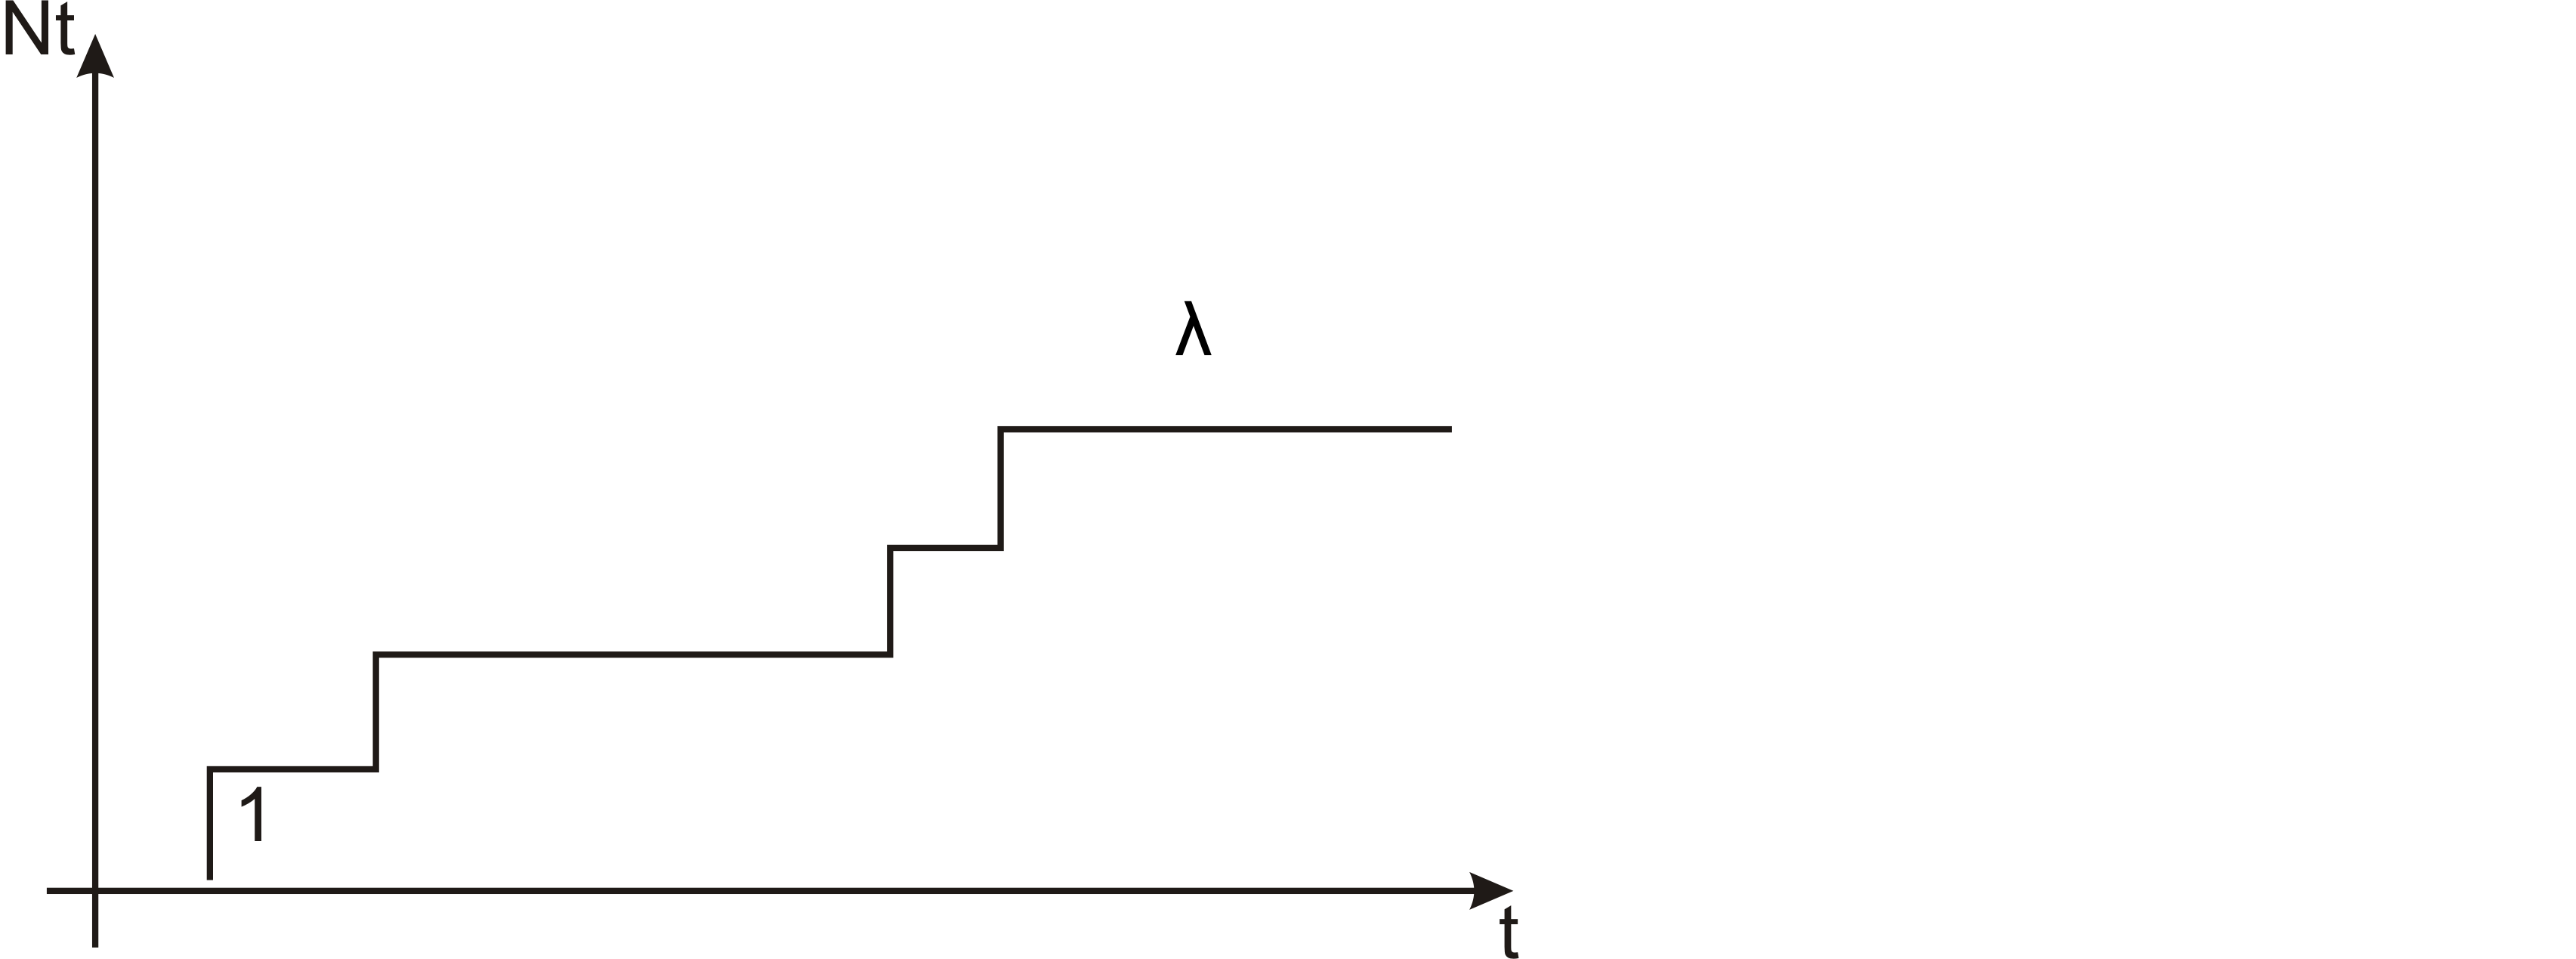
\includegraphics[width=4.5in]{Figures/rate.PNG}\\
 % \caption{}\label{}
\end{figure}
Suppose $\{N_{t}, t \geq 0\}$ Poisson process with rate $\lambda$. 

$\tilde{N_{t}}(w)= N_{t}(w)+f(t+X_{1}(w))$ where $f(t)$=0, if $t$ is irrational and $f(t)$=t, if $t$ is rational.\\
\begin{eqnarray*}
% \nonumber to remove numbering (before each equation)
  P[\tilde{N_{t}}\neq N_{t}] &= P[\omega:t+X_{1}(\omega) \text{is rational}],\\
  &= P[\omega:X_1(\omega)  \text{is rational} ] =0.
\end{eqnarray*}
 
\begin{eqnarray*}
% \nonumber to remove numbering (before each equation)
  P[\tilde{N_{t}}= N_{t}] &=& 1\\
  P[\tilde{N_{t_1}}= N_{t_1},\tilde{N_{t_2}}= N_{t_2} ] \\
  &=& \sum_{n_{1},n_{2}}P[\tilde{N_{t1}}= N_{t_1},\tilde{N_{t_2}}= N_{t_2}, N_{t_1}=n_1, N_{t_2}=n_2 ] \\
   &=& 1
\end{eqnarray*}
$\{\tilde{N_{t}}\}, \{N_{t}\}$ have same fdds.\\
$\{\tilde{N_{t}}(\omega)\}$ can take non-integer values and is not non-decreasing.\\
Two process can have same distribution but sample path behaviour can be quite different.\\


\section{Compound Poisson Process}
\begin{defn}[Compound Poisson process] Let $\left\{X_i\right\}$ be iid random variables. Let $N(t), t\geq 0$ be a Poisson Process with parameter $\lambda$ independent of $X_i, i\geq 1$. Then the process $X(t)$ defined as
\begin{equation*}
X(t) = \sum_{i=1}^{N(t)} X_i
\end{equation*}
is called a \textbf{compound Poisson process}.
\end{defn}
We derive some properties of compound Poisson Processes in the following.
\subsection{Mean}
\begin{align*}
E[X(t)] = E[\sum_{i=1}^{N(t)} X_i] &= E[E[\sum_{i=1}^{N(t)} X_i|N(t)]] \\
&= \sum_{k=0}^\infty E\left[\sum_{i=1}^{k} X_i|N(t)=k\right]\Pr\{N(t) = k\}\\
&= \sum_{k=0}^\infty \sum_{i=1}^{k} E[X_i]\Pr\{N(t) = k\}\\
&= E[N(t)]E[X_1] = \lambda tE[X_1].
\end{align*}

\subsection{MGF}
We leave it as an exercise to show that $M_{X(t)}(\theta)=E[e^{\theta X(t)}] = e^{(M_X(\theta)-1)\lambda t}$.

\subsection{A nice counterexample}
A Poisson process is not uniquely determined by it's distribution. Let $X_t = Y_t + f(Z+t)$, where $Y_t$ is a Poisson Process and 
\begin{equation*}
f(t) = t 1_{\{t \in \mathbb{Q}\}}.
\end{equation*}
Let $Z$ be a continuous random variable. Then we can show that $\Pr\{X_t \neq Y_t) = 0$. This is true since
\begin{flalign*}
\Pr\{X_t \neq Y_t\} &= \Pr\{\omega \in \Omega: \quad t+Z(w) \in \mathbb{Q}\} \\
&= P(Z \in \mathbb{Q}\setminus t) = 0
\end{flalign*}
The last part follows since $\mathbb{Q}\setminus t$ is a countable set of individual events with probability zero.
\end{document}